\section{一部と全部：分布と中心極限定理}

  \subsection{毎回変わってしまう待ち時間}

    話題のラーメン屋さんに行ってみると行列ができている.
    あなたは今このくらいの人数並んでいるからおおよそこのくらいの時間で自分の順番がくるだろうと考えて並ぶ.
    しかし, 実際のところその予想は当たらないことが大半だろう.
    すぐに行列が消化されてラッキーと思うこともあれば, 全然進まず別の店に行くか迷うこともある.
    とはいえ, 30人くらい並んでいたとしたら, 「絶対1時間以上待つだろう」と明らかにわかることもある.
    より正確に, それぞれの待ち時間がどのくらいの確率で起きるかを見積もるには, 人数や時間帯, 曜日などを加味してどのくらい待つものなのかたくさん経験してみるしかない.
    そうすると, 完全に正確な待ち時間をぴたりと当てることは難しいにせよ, おおまかな傾向はつかめるはずだ.
    このとき, 我々は「データの分布」というものを無意識のうちに考えている.
    たとえば100回通って取った待ち時間の記録がどのように分布しているかを確認することによって,
    その背後にある, 全ての記録を含むような神様しか知らない「本当の分布」から計算される, それぞれの待ち時間がどのくらいの確率で起きるかを見積もっているのだ.

  \subsection{手元のデータとその出どころ}

    ラーメン屋に100回通って取った記録から平均を出したとしても, 別の100回ならその平均も少し違う数になるだろう.
    前の章の終わりに残った, 映画80本の疑問もこれと同じだ.
    手元の80本を平均すれば $209.4$ 万回になることは間違いないが, 別の80本でもそうなるとは限らない.
    大ヒット作が多めに入って $230$ 万回になるかもしれないし, そうした作品が少なくて $190$ 万回に下がるかもしれない.
    計算を何度やり直しても答えは同じなのに, 計算する相手を取り直すと答えが変わってしまうのである.

    この手元にある分と, その背後にある全部とを区別するために, 名前をつけておこう.

    \begin{defi}{母集団と標本}{population-sample}
      調査や分析の対象となる集まり全体を\textbf{母集団}と呼ぶ.
      その母集団から実際に観測するために取り出された一部のデータを\textbf{標本}と呼び,
      標本に含まれるデータの個数を\textbf{標本サイズ}と呼ぶ.
    \end{defi}

    映画なら, その配信サービスで配信されている対象作品全体が母集団で, 手元の80本が標本になる.
    標本サイズは $n = 80$ だ.
    本当は全部の様子を知りたいのだが, 全部を調べるのは難しいので, 一部を使って見当をつけようとしている.
    待ち時間の記録から本当の分布を考えたのと, やっていることは同じである.

    ただ, 一部なら何でもよいというわけにはいかない.
    ランキング上位の人気作ばかり80本集めてきたら, 平均が高くなるのは当たり前だろう.
    足し算も割り算も正しくできているのに, 作品全体の様子からは離れてしまう.
    我々は計算を始める前に, すでに大事なことを決めてしまっているのだ.
    以下では, この80本は対象作品全体から大きな偏りなく選ばれた標本として扱うことにする.

  \subsection{偏ったサイコロの平均}

    さて, 取り直せば平均が変わることはわかったが, どれくらい変わるものなのだろうか.
    元のデータが極端に偏っていれば, 平均の分布も同じように偏りそうな気がする.
    そもそもそのデータを足して割っただけなのだから, そう思うのも無理はない.
    サイコロで試してみよう.

    使うのは, 1の目が出る確率が $50\%$ で, 2から6の目はそれぞれ $10\%$ ずつしか出ないサイコロだ.
    ふつうのサイコロならどの目も同じ確率で出て, 理論上の平均は3.5になる.
    こちらは1が半分を占めるので, 理論上の平均は2.5だ.
    出目の確率を棒で描くと, 1のところだけが高く, あとは平らに並ぶ形になる.
    これがこのサイコロの本当の分布である.
    ラーメン屋の待ち時間と違って, 今回は我々が確率を決めたので, 神様の側から先に形を知っているわけだ.

    このサイコロを5回振り, 出た目を足して5で割る.
    それだけでは平均は一つしか出てこないので, 「5回振って平均を出す」ところまでを1000回繰り返してみる.
    こうして集まった1000個の平均を, ヒストグラムにする.
    さらに, 5回を30回に増やして同じことをやってみたのが\cref{fig:ch03-dice-clt}だ.

    \begin{figure}[htbp]
      \centering
      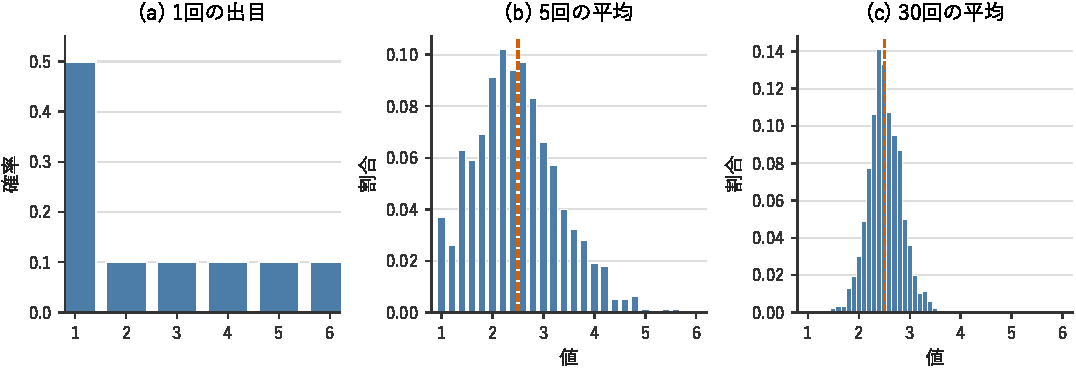
\includegraphics[width=\linewidth]{../figures/output/ch04_dice_clt.pdf}
      \caption{偏ったサイコロの出目と標本平均の分布. 破線は理論上の平均2.5. 5回または30回振って平均を取る操作を1000回ずつ繰り返した. 5回の平均は0.2刻みの値しか取らないため, (b)の棒は櫛状に並ぶ.}
      \label{fig:ch03-dice-clt}
    \end{figure}

    (a)では1の棒だけが高かったのに, 5回の平均を集めた(b)には, まだ少し左に偏っているものの, なだらかな山が現れている.
    30回の平均を集めた(c)では, 2.5を中心にした左右対称の釣鐘型にかなり近くなった.
    サイコロをまともなものに取り替えたわけではない.
    相変わらず半分は1が出るサイコロを振っているのに, 30個を足して割るだけで, 平均の分布は元の出目と似ても似つかない形になっている.
    平均を取るというのは, ずいぶん面白いことをしていたのである.

  \subsection{標本分布と中心極限定理}

    今の実験では, 振るたびに出てくる目を数える代わりに, 何回か振るたびに出てくる平均を数えた.
    前の章でたくさんの値を一つにまとめたばかりなのに, その一つの数も集め直せばまたたくさんになって, 分布が描ける.
    この分布にも名前がついている.

    \begin{defi}{標本分布}{sampling-dist}
      母集団から標本を繰り返し取り直し, そのたびに統計量を計算するとき, その統計量の値が従う確率分布を, その統計量の\textbf{標本分布}と呼ぶ.
    \end{defi}

    名前に「標本」と入っているが, 標本分布は手元にあるデータそのものの分布ではない.
    サイコロの図の(a)は, 振る前から決まっている出目の本当の分布だった.
    (b)と(c)は, 標本を取り直しては平均を計算することを繰り返して描いた, 平均の標本分布の様子なのである.

    サイコロの平均が釣鐘型に近づいたのは, たまたまうまい具合に目が出たからではない.
    振る回数を増やすとどうなるかについて, 次のことがわかっている.

    \begin{thm}{中心極限定理}{clt}
      平均 $\mu$, 分散 $\sigma^2$ をもつ同一の分布から, 互いに独立に $n$ 個の値を取り出し, その標本平均を $\bar{X}$ とする.
      $n$ が大きくなるにつれて, $\bar{X}$ の標本分布は正規分布 $N\!\left(\mu,\; \sigma^2 / n\right)$ に近づく.
    \end{thm}

    同じ分布から互いに独立に値を取り出すことを, \textbf{独立同分布}という.
    サイコロなら, 毎回同じサイコロを, 前の出目とは関係なく振るということだ.
    この条件のもとでは, 元の分布が釣鐘型でなくてもよい.
    段差のあるサイコロでも, 右に裾を引く映画の視聴回数でも, 平均を作る個数 $n$ を増やせば, 平均の分布は釣鐘型に近づいていく.
    「$n$ が大きくなるにつれて」とあるのは, 少ない個数でもぴったり同じ形になると言っているわけではないからだ.
    どのくらいの速さで近づくかは, 元の分布によって違う.

    この釣鐘型が\textbf{正規分布}で, 中心の平均値 $\mu$ と, 散らばりの大きさを表す標準偏差で形が決まる.
    平均値から左右に標準偏差2つ分の範囲を取ると, 全体の約 $95\%$ が入るという性質がある.
    形がわかるというのは, どこにどれくらい集まるかまでわかるということなのだ.

    さらに定理の式には, サイコロの図でも見えていたことがもう一つ書かれている.
    平均の分布の分散は, 元の値の分散 $\sigma^2$ を $n$ で割った $\sigma^2/n$ になる.
    個数を増やすと釣鐘型に近づくだけでなく, 中心の $\mu$ のまわりに狭く集まってくるのである.

    \begin{mybox}{分布という言葉について}
      前の章では, データがどのあたりに多く集まり, どこに少ないかという全体の姿を「分布」と呼んだ.
      ところが今は, 振る前のサイコロにも, 取り直した平均にも同じ言葉を使っている.
      手元のデータの話だったはずなのに, いつの間にか話が広がっているではないか.
      「分布」は形を指す言葉で, 何の形なのかは, 何を数えているかで決まるのである.

      映画80本のヒストグラムは, 視聴回数の区間ごとに作品を数えた記録の分布で, 前の章の意味そのままだ.
      サイコロの図の(a)は, どの目がどの確率で出るかという本当の分布である.
      1が $50\%$ という決まりは振る前からあり, 手元に記録があってもなくても変わらない.
      そして(b)(c)で数えたのは, 取り直すたびに計算した平均だ.
      どれも棒の絵で描けるが, 記録, 本当の分布, 統計量の分布, つまり本文で標本分布と呼んだものと, 描いているものが違っている.

      まず, 記録は本当の分布から得た一部分で, 偏りなく記録を増やせば, ヒストグラムの形は本当の分布に近づいていく.
      だから手元の80本を, 全体の代役にしてみることもできるわけだ.
      次に, 統計量の分布は, 本当の分布と標本サイズ $n$, それにどんな計算をするかで決まる.
      サイコロの(a)から30回分を取って平均を作ると(c)になる, というのがその実例である.

      では, 正規分布という釣鐘型はどこに出てくるのだろうか.
      これは形につけた名前なので, 三つのどこに現れてもよい.
      同じ分布から独立に取った値を足すと釣鐘型に近づく, というのが中心極限定理の言っていることで, 平均も足し算をしているから釣鐘型に近づく.
      身長のように, 同じ分布とは限らない多くの要因が足し合わさったものにも似た性質が知られていて, 身長の形が釣鐘型に近いのはそのためだと説明される.
      ただし, この本では, データそのものが正規分布だとは仮定しない.
      正規分布を使うのは, 平均やその差といった統計量が, 取り直したときにどんな分布になるかを考える場面だけだ.

      本当の分布は, 調べる相手によって形が違う.
      ふつうのサイコロならどの目も同じ確率の一様分布, 同じ確率で独立に当たり外れを繰り返したときの当たりの回数なら二項分布が出てくる.
      めったに起きないことの回数にはポアソン分布, 測定値などには釣鐘型の正規分布が使われることもある.
      もっとも, 映画の本当の分布はこのどれでもなく, 右に裾を引いた形だ. 本当の分布に名前があるとは限らないのである.

      一方, 本当の分布がどんな形でも, 平均は $n$ を大きくすると正規分布に近づく.
      正規分布から取ったデータなら, 平均が本当の平均からどれだけずれているかを, 分からない $\sigma$ の代わりに手元のデータから計算した標準偏差を使って測ると, その数は正規分布ではなく $t$ 分布という親戚に従う.
      $n$ が大きければ正規分布と見分けがつかない. 後の章の検定で名前が出てくる.
      同じく正規分布から取ったデータなら, 手元のデータから計算した分散がどんな分布になるかも分かっていて, 尺度を除けばカイ二乗分布と呼ばれる形になる. これも正規分布から作られた親戚である.
      独立に見積もった二つの分散の比を扱う親戚には $F$ 分布もあるが, カイ二乗分布と $F$ 分布はこの本の本文では使わない.

      正規分布が本当の分布と統計量の分布の両方に現れる理由は, 足し算にある.
      二項分布が試行回数 $n$ を増やすと正規分布に近づくのも, 当たりか外れかを足しているからで, その平均に中心極限定理を当てたのと同じことだ.
      本当の分布の形はいろいろだが, この本で扱う統計量の形は, 正規分布とそこから作られた親戚でほとんど足りる.
      この本で先に出てくる分布の名前はこれで全部である.
    \end{mybox}

  \subsection{平均のばらつきを計算する}

    分散が $\sigma^2/n$ なら, 平方根を取った標準偏差は $\sigma/\sqrt{n}$ だ.
    これが, 取り直したときに平均がどれくらい動くかを表す数になる.
    平均を何度も取り直して並べなくても, 元の値の標準偏差と個数から計算できてしまう.

    \begin{defi}{標準誤差}{se}
      母集団の標準偏差を $\sigma$, 標本サイズを $n$ とするとき, 標本平均の\textbf{標準誤差}（SE: Standard Error）を
      \[
        \mathrm{SE} = \frac{\sigma}{\sqrt{n}}
      \]
      と定義する.
    \end{defi}

    とはいえ, このままでは少し困る.
    分子の $\sigma$ は本当の分布の標準偏差なのに, 我々はその全部を調べられないから一部を使っていたのだった.
    そこで, 手元の標本から計算した標準偏差に代役を頼むことにする.

    ただし, 前の章で使った分散 $s^2$ をそのまま使うのではなく, 割る数を $n$ から $n-1$ に変える.

    \[
      u^2 = \frac{1}{n-1}\sum_{i=1}^{n}(x_i-\bar{x})^2, \qquad u = \sqrt{u^2}
    \]

    この $u^2$ を\textbf{不偏分散}といい, その平方根 $u$ で本当の標準偏差を見積もる.
    手元のデータ自身をまとめるときと, その背後にある全部のばらつきを見積もるときとで, 割る数が少し違うのである.
    なぜそうするのかはこの節の終わりのコラムに譲って, 今はこの $u$ を使って計算を進めよう.
    実際に手元で計算する標準誤差は,
    \[
      \mathrm{SE} = \frac{u}{\sqrt{n}}
    \]
    となる.

    標準偏差と標準誤差は名前がよく似ているので, どちらも同じようなものに思えるかもしれない.
    しかし $u$ が見ているのは一本一本の映画の違いで, 標準誤差が見ているのは, 映画を選び直すたびに出てくる平均の違いだ.
    本数を増やしたからといって, 大ヒット作とほとんど見られない作品との差が縮まるわけではない.
    だから個々の値のばらつきを見積もる $u$ は, データを増やしてもそれだけで小さくはならない.
    一方, 標準誤差には分母に $\sqrt{n}$ があるので, 本数を増やすと小さくなる.
    一本一本の違いは大きいままでも, まとめて平均を取ると, 取り直しによる違いを小さくできるのである.

    \begin{mybox}{なぜ $n-1$ で割るのか}
      分散を計算するとき, データの記述では個数 $n$ で割っていたのに, 母集団の分散を見積もるときには $n-1$ で割った.
      この「1を引く」ことにはどんな意味があるのだろうか.

      手元にあるデータから分散を計算するとき, 本当なら母集団全体の真の平均 $\mu$ からのずれを測りたい.
      ところが $\mu$ は分からないので, 代わりに手元の標本平均 $\bar{x}$ を使って $(x_i - \bar{x})^2$ を計算する.

      $\bar{x}$ は, 手元にあるデータのちょうど真ん中に来るように作った値だ.
      データ自身の平均からのずれを二乗して足し合わせると, ほかのどんな基準値を使ったときよりも合計が小さくなってしまう性質がある.
      真の平均 $\mu$ は手元の $\bar{x}$ と少しずれた場所にあるはずなので, $\bar{x}$ から測った二乗の合計は, $\mu$ から測ったときより小さめに出てしまう.

      その分を補正するために, 分母の $n$ を少し小さくして $n-1$ で割っている.
      手元のデータ数が80件なら, $n$ で割るのと $n-1$ で割るのとで結果の差はごくわずかだが, 理屈の上ではこのような差の調整が行われている.
    \end{mybox}

  \subsection{映画の平均はどれくらい動くか}

    それでは, 映画でもサイコロと同じことが起きるのか, 試してみよう.
    対象作品全体から80本を何度も取り直せればよいのだが, 手元にあるのは今の80本だけだ.
    ひとまずこれを全体の代役にして, その中からランダムに20本を選んで平均を出すことにする.
    一度選んだ作品は候補に戻してから次の1本を選ぶ. これを復元抽出という.
    同じ作品がまた選ばれることもあるが, こうしておけば, 前に何を選んだかで次の候補が変わらずにすむ.
    「20本を選んで平均を出す」ところまでを1000回繰り返して, 1000個の平均を並べてみる.

    もちろん, この実験で選べるのは, あくまで手元にある作品だけである.
    全体から取り直すことを完全に再現しているわけではないが, 平均がどう動くかの見当はつけられる.

    \begin{figure}[htbp]
      \centering
      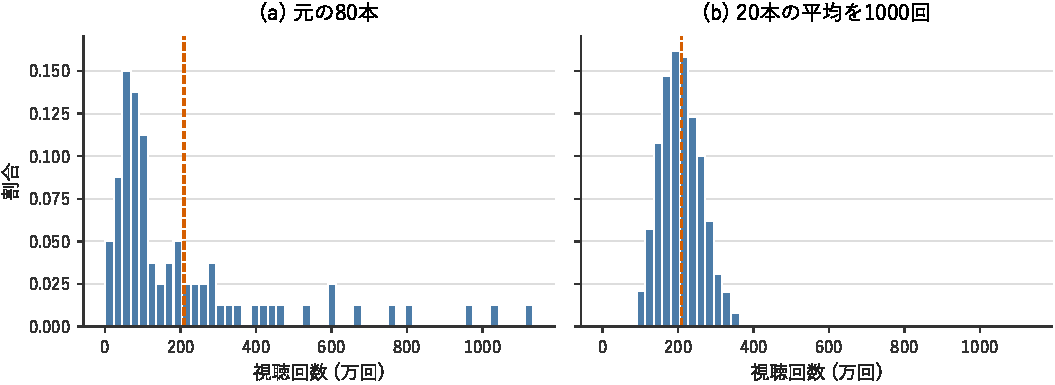
\includegraphics[width=\linewidth]{../figures/output/ch04_sampling_dist.pdf}
      \caption{元の映画80本の視聴回数と, 80本から20本を復元抽出して求めた標本平均の分布. 復元抽出と平均の計算を1000回繰り返した. 横軸と縦軸の尺度は左右で共通で, 破線は80本全体の平均を示す.}
      \label{fig:ch03-sampling-dist}
    \end{figure}

    \cref{fig:ch03-sampling-dist}の左は, 元の80本の視聴回数だ.
    右に長い裾を引いていた形が, 20本ずつの平均を1000回集めた右の図では, 左右対称の釣鐘型にかなり近くなっている.
    選べる作品は左の図にあるものだけなのに, 平均を計算して並べると, こんなに違う姿になるのだ.
    左右で横軸の目盛りをそろえてあるので, 平均の散らばる幅がずっと狭くなっていることもわかる.

    さて, 今の実験は20本の平均だったが, 知りたかったのは80本の平均 $209.4$ 万回がどれくらい動くかだった.
    もう一度実験をしなくても, 今度は標準誤差の式で計算できる.
    標本サイズは $n = 80$ で, $n-1 = 79$ で割って求めた標準偏差 $u$ はおよそ $240.8$ 万回になる.
    前の章で $n = 80$ で割って求めた $s$ は $239.3$ 万回だったので, 少しだけ大きくなった.
    $\sqrt{80} \approx 8.94$ を使うと,

    \[
      \mathrm{SE} = \frac{u}{\sqrt{80}} \approx \frac{240.8}{8.94} \approx 26.9
    \]

    となり, 標準誤差はおよそ $26.9$ 万回だ.
    先ほどの20本から80本へと本数が4倍になると, 分母は $\sqrt{4} = 2$ 倍になる.
    つまり, 平均のばらつきは20本のときの半分ほどになる計算だ.
    本数を増やすのは大変なのに, ばらつきが小さくなるのは, その平方根の分だけなのである.

    一本一本の映画は, 何百万回も見られる作品からほとんど見られない作品まであって, 標準偏差でいえば $240$ 万回も散らばっていた.
    それが80本の平均になると, 別の80本を取り直したときのばらつきは, 標準誤差でおよそ $27$ 万回になる.
    最初の $209.4$ 万回という数だけではわからなかった, 取り直すとどれくらい動くかという大きさまで, 手元の80本だけから計算できたのである.

  \begin{mybox}{ここまででわかったこと}
    四段階の三つ目「ばらつきを見積もる」.

    \textbf{この章で言えるようになったこと}: 一本一本の映画は標準偏差で約 $240$ 万回も散らばるが, 80本の平均を取り直したときのばらつきは, 標準誤差で約 $27$ 万回と見積もれた.
    対象作品全体から大きな偏りなく選ばれた標本として扱えば, 手元の80本だけからこれを計算できる.

    \textbf{まだ言えないこと}: 取り直した平均がどれくらい動くかはわかったが, 作品全体の本当の平均はどのあたりにあるのだろうか.

    \textbf{前の章の見方がどう変わったか}: 手元の80本が決まれば, 平均は $209.4$ 万回に決まる.
    だが, 別の80本を集めれば, その一つの数も変わる.
  \end{mybox}
